%!TEX root = ../main.tex

\chapter{Reti di Hopfield} % (fold)
\label{cha:reti_di_hopfield}
Si passa ora allo studio delle reti neurali viste come sistemi dinamici non lineari, con particolare attenzione al problema della loro stabilità o neurodinamica (vedi Appendice~\ref{cha:sistemi_dinamici}). Un modo implicito per introdurre in una rete neurale la variabile tempo è mediante l’utilizzo di reti con feedback o ricorrenti.

\section{Modello di Hopfield: caso discreto} % (fold)
\label{sec:modello_di_hopfield_caso_discreto}

Le reti ricorrenti con unità non lineari sono generalmente difficili da analizzare.  Possono comportarsi in modi differenti: convergere a uno stato stabile, oscillare o seguire \emph{traiettorie caotiche} il cui andamento non è prevedibile.\\

Tuttavia, il fisico americano \emph{John Hopfield} (e altri gruppi) si accorsero che se le connessioni sono \textbf{simmetriche} esiste una \emph{funzione di energia globale}.\\

Le reti di Hopfield sono dunque:
\begin{itemize}
	\item \textbf{reti ricorrenti ad uno strato} in cui ogni neurone è connesso a tutti gli altri (sono assenti
	connessioni con se stesso), quindi $w_{ii}=0$;
	\item \textbf{simmetriche}: perché hanno la matrice dei pesi sinaptici simmetrica, ovvero $W=W^T$;
	\item \textbf{non lineari}: ogni neurone ha una funzione di attivazione non lineare invertibile.
\end{itemize}

\begin{figure}[h!]
	\centering
	\begin{tikzpicture}[->,>=stealth',shorten >=1pt,auto,node distance=4cm, semithick]
		\tikzstyle{every state}=[align=center, fill=blue!20,draw=blue]
		
		% Draw nodes.
		\node[state] (1) {$1$};
		\node[state, right of=1] (2) {$2$};
		\node[state, right of=2] (N) {$N$};
        
		% Draw edges
		\path 
		(1) edge[bend left, below] node {$w_{12}$} (2)
		(1) edge[bend left] node {$w_{1N}$} (N)
		(2) edge[bend left] (1)
		(2) edge[bend left] (N)
		(N) edge[bend left] (1)
		(N) edge[bend left] (2)
		(2) edge[dotted, -] (N);
        
	\end{tikzpicture}
	\caption{Una rete ricorrente.}
\end{figure}

\newpage

Per quanto riguarda l'aggiornamento di un neurone si possono scegliere tre strade diverse:
\begin{enumerate}
	\item \textbf{aggiornamento asincrono}: in cui si aggiorna un neurone alla volta;
	\item \textbf{aggiornamento sincrono}: tutti i neuroni vengono aggiornati allo stesso istante;
	\item \textbf{aggiornamento continuo}: in cui tutti i neuroni si aggiornano continuamente.
\end{enumerate}

In questa sezione saranno trattate le reti di Hopfield nel caso in cui il tempo scorra in maniera discreta e i neuroni si aggiornino in modo asincrono.\\

Nel caso discreto si adotta lo stesso modello di McCulloch e Pitts con l'aggiunta di un fattore esterno che influenza l'input al neurone $i$.
\begin{align}
	H_i = \underbrace{\sum_{j \neq i} w_{ij} V_j}_\textrm{modello M\&P} + \underbrace{I_i}_\textrm{input esterno}
\end{align}
E l'output di ogni neurone è così definito:
\begin{align}
	V_i =
	\begin{cases}
		+1, &\text{ se } H_i \geq 0\\
		-1, &\text{ se } H_i < 0
	\end{cases}\label{eq:learningrule}
\end{align}
L'aggiornamento dei neuroni è un processo casuale. Per selezionare il neurone da aggiornare si può procedere in due modi:
\begin{enumerate}
	\item ad ogni istante temporale si sceglie a caso l'unità $i$ da aggiornare (utile nelle simulazioni);
	\item Ogni unità si aggiorna indipendentemente con probabilità costante ad ogni istante.
\end{enumerate}

\newpage

A differenza delle reti feed-forward quelle di Hopfield sono sistemi dinamici. La rete parte da uno stato iniziale
\begin{align*}
	V(0) = (V_1(0), \dots, V_n(0))^T
\end{align*}

e si evolve lungo una traiettoria fino a raggiungere un punto fisso in cui $V(t+1) = V(t)$ (convergenza).
\begin{figure}[h!]
	\centering
	\begin{tikzpicture}
		\node[point] (0) at (-4, 0) {};
		\node[point] (1) at (-2, 2) {};
		\node[point] (2) at (0, -0.4) {};
		\node[point] (3) at (2, 1) {};
		\node[point] (4) at (4, 0) {};
		\node[point] (5) at (6, -0.5) {};
		\node[point] (6) at (8, 0.5) {};
         
		\foreach \x / \y in {0/1,1/2,2/3,3/4,4/5,5/6}
		\path (\x) edge[->] (\y);
         
		\foreach \x in {0,...,6}
		\node[above=2mm of \x] {\small$V(\x)$};
         
	\end{tikzpicture}
	\caption{Traiettoria di una rete di Hopfield}
\end{figure}

\subsection{La funzione energia} % (fold)
\label{sub:funzione_energia}
Si procede ora allo studio del comportamento di una rete di Hopfield; fino ad ora infatti non è stato dimostrato se la rete converge oppure produce cicli. Il sistema è governato da una funzione di energia $E$. L'energia globale è la somma di una serie di contributi locali. Ogni contributo dipende da \textbf{una} connessione $w_{ij}$ e dagli stati binari dei \textbf{due} neuroni $V_i V_j$. La funzione energia è dunque così definita:
\begin{align}
	E = - \frac{1}{2} \sum_{i=1}^n \sum_{\substack{j=1 \\ j \neq i}}^n w_{ij} V_i V_j - \sum_{i=1}^n I_i V_i\label{eq:energy}
\end{align}
Dove $I$ è il fattore esterno (termine bias) e coinvolge lo stato di un'unità individualmente. Il fattore $1 / 2$ è aggiunto perché i termini identici $w_{ij}x_i x_j$ e $w_{ji} x_j x_i$ sono presenti nella doppia sommatoria. Questa funzione permette ad ogni unità di calcolare \textbf{localmente} come il suo cambio di stato influenza l'energia globale. In termini matematici la differenza di energia è definita nel seguente modo:
\begin{align}
	\emph{Energy gap }\Delta E = E(t + 1) - E(t)
\end{align}
% subsection funzione_energia (end) 

\newpage

\subsection{Teorema di Hopfield nel caso discreto} % (fold)
\label{sub:teorema_di_hopfield_nel_caso_discreto}
Si enuncia ora una condizione sufficiente alla convergenza del sistema.
\begin{thm}[Terorema di Hopfield - Caso discreto]
	Se la matrice dei pesi di una rete di Hopfield è:
	\begin{enumerate}
		\item simmetrica: $W=W^T$;
		\item gli elementi lungo la diagonale di $W$ sono nulli: $diag(W) = 0$.
	\end{enumerate}
	Allora la funzione di energia:
	\begin{align*}
		E = - \frac{1}{2} \sum_{i=1}^n \sum_{\substack{j=1 \\ j \neq i}}^n w_{ij} V_i V_j - \sum_{i=1}^n I_i V_i
	\end{align*}
	è una funzione di Lyapunov per il sistema. E quindi:
	\begin{align*}
		\Delta E = E(t+1) - E(t) < 0
	\end{align*}
	dove $\Delta E = 0$ solo quando il sistema ha raggiunto un punto stazionario.
\end{thm}

\begin{proof}[Dimostrazione:]
	Assumendo che i neuroni si aggiornano in modo asincrono, supponiamo che il neurone $h$ cambi il proprio stato. La differenza di energia è data da:
	\begin{align*}
		\Delta E &= - \frac{1}{2} \sum_{i=1}^n \sum_{\substack{j=1 \\ j \neq i}}^n w_{ij} V_i(t + 1) V_j(t + 1) - \sum_{i=1}^n I_i V_i(t + 1) \\
		&+ \frac{1}{2} \sum_{i=1}^n \sum_{\substack{j=1 \\ j \neq i}}^n w_{ij} V_i(t) V_j(t) + \sum_{i=1}^n I_i V_i(t) \\
		&= \underbrace{- \frac{1}{2} \sum_{i=1}^n \sum_{\substack{j=1 \\ j \neq i}}^n w_{ij} \cdot [V_i(t + 1) V_j(t + 1) - V_i(t) V_j(t)]}_\textbf{$A$} \\
		& \underbrace{- \sum_{i=1}^n I_i \cdot [V_i(t + 1) - V_i(t)]}_\textbf{$B$}
	\end{align*}
    
	\newpage
    
	Si consideri il secondo termine $B$:
	\begin{align*}
		B = - \sum_{i=1}^n I_i \Delta V_i
	\end{align*}
	ora dal momento che $h$ è l'unico stato che è cambiato abbiamo che
	\begin{align*}
		B = - I_h \Delta V_h
	\end{align*}
	in quanto tutti gli altri $\Delta$ sono uguali a 0.\\
    
	Si passa ora al primo termine $A$. Si espande la sommatoria isolando il neurone $h$:
	\begin{align*}
		A &= \underbrace{- \frac{1}{2} \sum_{i \neq h} \sum_{j \neq i} w_{ij} \cdot [V_i(t + 1) V_j(t + 1) - V_i(t) V_j(t)]}_\textrm{$A_1$} \\
		& \underbrace{- \frac{1}{2} \sum_{j \neq h} w_{hj} \cdot [V_h(t + 1) V_j(t + 1) - V_h(t) V_j(t)]}_\textrm{$A_2$}
	\end{align*}
	Dal momento che solo il neurone $h$ cambia stato allora $V_i(t) = V_i(t + 1)$ per $i \neq h$ quindi $A_1$ può essere riscritto nel seguente modo:
	\begin{align*}
		A_1 &= - \frac{1}{2} \sum_{i \neq h} \sum_{j \neq i} w_{ij} \cdot [\underbrace{V_i(t + 1)}_\textrm{$=V_i(t)$} V_j(t + 1) - V_i(t) V_j(t)] \\
		&= - \frac{1}{2} \sum_{i \neq h} \sum_{j \neq i} w_{ij} \cdot V_i(t) \underbrace{[V_j(t + 1) - V_j(t)]}_\textrm{$=\Delta V_j$} \\
		&\text{A questo punto $\Delta V_j \neq 0$ solo quando $j = h$ quindi $\Delta V_j = \Delta V_h$} \\
		&= - \frac{1}{2} \sum_{i \neq h} w_{ih} V_i(t) \Delta V_h
	\end{align*}
	Per quanto riguarda $A_2$ il procedimento è lo stesso:
	\begin{align*}
		A_2 &= - \frac{1}{2} \sum_{j \neq h} w_{hj} \cdot [V_h(t + 1) V_j(t + 1) - V_h(t) V_j(t)] \\
		&= - \frac{1}{2} \sum_{i \neq h} w_{hi} V_i(t) \Delta V_h
	\end{align*}
	Siccome la matrice dei pesi è simmetrica $W = W^T$ allora $w_{ih} = w_{hi}$ e quindi:
	\begin{align*}
		A = A_1 + A_2 = - \Delta V_h \sum_{i \neq h} w_{ih} V_i(t)
	\end{align*}
	
	In questo modo si ottiene:
	\begin{align*}
		\Delta E &= - \Delta V_h \sum_{i \neq h} w_{ih} V_i(t)  - I_h \Delta V_h \\
		&= - \Delta V_h \underbrace{\left[\sum_{i \neq h} w_{ih} V_i(t) + I_h \right]}_\textrm{input di $h$ al tempo $t + 1$} \\
		&= - \Delta V_h \cdot H_h
	\end{align*}
	A questo punto è necessario dimostrare che il prodotto $\Delta V_h \cdot H_h$ è sempre positivo in modo tale da provare la tesi, ovvero che $\Delta E \leq 0$. Per la regola di apprendimento \eqref{eq:learningrule}:
	\begin{enumerate}
		\item se $V_h > 0 \Leftrightarrow H_h \geq 0$
		\item se $V_h < 0 \Leftrightarrow H_h < 0$
	\end{enumerate}
	Dunque il prodotto è sempre positivo C.V.D.
\end{proof}
% subsection teorema_di_hopfield (end)

% section modello_di_hopfield_caso_discreto (end)

\newpage

\section{Regola di Hebb}
Nei computer se si vuole accedere ad una certa informazione si utilizza il suo preciso indirizzo di memoria. Questo tipo di memoria è definita \emph{byte-addressable memory}. Nel cervello umano, invece, la memoria è indirizzata in base al contenuto, \emph{content-addressable memory}. Ad esempio pensare alla parola “volpe” potrebbe automaticamente attivare memorie relative ad altri animali simili, alla caccia, oppure al concetto di furbizia.\\

In questo contesto, è stata introdotta la \emph{regola di Hebb} per descrivere questo meccanismo di accesso alle informazioni. L'apprendimento Hebbiano si basa sul semplice principio che se due neuroni si attivano contemporaneamente, la loro interconnessione deve essere rafforzata. In dettaglio il postulato di Hebb afferma che:\\

\emph{Quando un assone di un neurone A è abbastanza vicino da eccitare un neurone B e questo, in modo ripetitivo e persistente, gli invia un potenziale di azione, inizia un processo di crescita in uno o entrambi i neuroni tali da incrementare l'efficienza di A.}\\

In termini matematici la memoria è rappresentata da un insieme di $p$ patterns $x^\mu$, con $\mu=1,\dots,p$. Quando viene presentato un nuovo pattern $x$, la rete risponde producendo il patern salvato in memoria che più assomiglia ad $x$.\\

Hebb suggerisce variazioni sull'efficacia sinaptica proporzionali alla correlazione nell'attivazione tra un neurone pre e post sinaptico.
\begin{align}
	w_{ij} = \frac{1}{N} \sum_{\mu = 1}^p x_i^\mu x_j^\mu
\end{align}
dove $N$ è il numero di unità binarie con output $s_1, \dots, s_N$

Si consideri il seguente esempio con due pattern che la rete ha imparato:
\begin{align*}
	x^1 = (-1,-1,-1,+1) \\
	x^2 = (+1,+1,+1,+1)
\end{align*}
I pesi sono cosi calcolati:
\begin{align*}
	w_{ij} = \frac{1}{4} \sum_{\mu=1}^2 x_i^\mu x_j^\mu
	\end{align*} 
	Ad esempio:
	\begin{align*}
		w_{12} = \frac{1}{4}(x^1_1 \cdot x^1_2 + x^2_1 \cdot x^2_2) = 
		\frac{1}{4}(-1 \cdot -1 + 1 \cdot 1) = \frac{1}{4} \cdot 2
	\end{align*}
	E quindi la matrice dei pesi ha la seguente forma:
	\begin{align*}
		W = \frac{1}{4} \cdot
		\begin{bmatrix}
			2 & 2 & 2 & 0 \\
			2 & 2 & 2 & 0 \\
			2 & 2 & 2 & 0 \\
			0 & 0 & 0 & 2
		\end{bmatrix}
	\end{align*}
	Si ricorda che l'output dell'unità $i$ è dato da:
	\begin{align*}
		s_i = Sgn \left(\sum_j w_{ij} s_j \right)
	\end{align*}
	Ad esempio dato l'input $(-1,-1,-1,+1)$ la rete produce il seguente output:
	\begin{align*}
		s_1 &= Sgn \left( \frac{1}{4} \cdot
		\begin{bmatrix}
			2 & 2 & 2 & 0 \\
			2 & 2 & 2 & 0 \\
			2 & 2 & 2 & 0 \\
			0 & 0 & 0 & 2
			\end{bmatrix} \cdot (-1, -1, -1, +1)^T \right) \\ 
			&= Sgn(-1.5, -1.5, -1.5, 0.5) = (-1,-1,-1,+1)
		\end{align*}
		Ed è una soluzione stabile in quanto corrisponde ad uno dei pattern memorizzati dalla rete, mentre il seguente esempio è una soluzione spuria:
		\begin{align*}
			input^2 = (-1,-1,-1,-1)&\longrightarrow output^2 = (-1,-1,-1,-1) \tag{spuria}
		\end{align*}


		\newpage


		\section{Modello di Hopfield: caso continuo} % (fold)
		\label{sec:modello_di_hopfield_caso_continuo}
		In questo modello i neuroni non sono più dispositivi binari con stati (0,1) o (-1,1), ma assumono un numero reale che identifica la quantità di corrente elettrica. Lo scopo di Hopfield era infatti quello di fornire un'implementazione fisica del suo modello e che imiti il più possibile il funzionamento di un cervello biologico.\\

		In questo caso, l'output di un neurone $i$ è il seguente:
		\begin{align}
			V_i = g_\beta(\mu_i) = g_\beta \left(\sum_{j} w_{ij} V_j + I_i \right) \qquad \text{oppure } \mu_i = g^{-1}_\beta(V_i) \label{eq:vi}
		\end{align}
		dove $g_\beta$ è la funzione di attivazione crescente, continua e non lineare. Le funzioni più utilizzate come $g$ sono la tangente iperbolica e la sigmoidea:
		\begin{align*}
			\tanh_\beta \mu = \frac {e^{\beta\mu} - e^{-\beta\mu}} {e^{\beta\mu} + e^{-\beta\mu}} \quad\in ]-1,1[
			\qquad\qquad
			g_\beta(\mu) =\frac{1}{1 + e^{- \beta \mu}} \quad\in ]0,1[
		\end{align*}

		Il parametro $\beta$ indica la “stickiness” della funzione. Ad esempio con $\beta \rightarrow \infty$ la funzione diventa sempre più ripida fino a diventare lineare.\\

		\begin{figure}[h!]
			\centering
			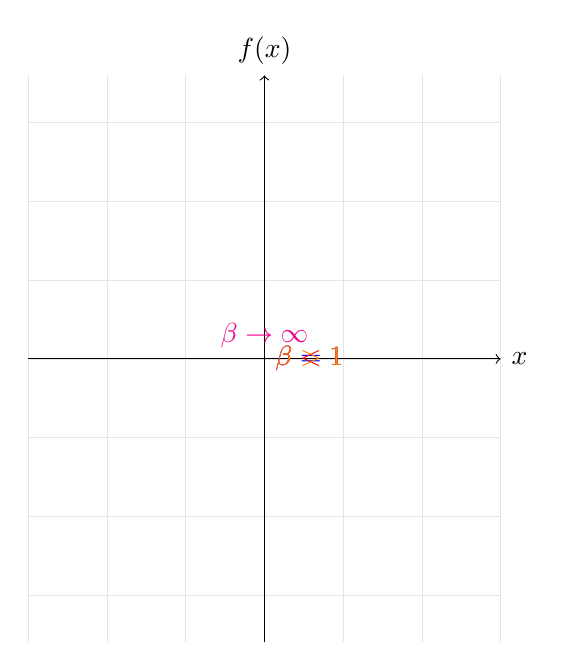
\begin{tikzpicture}[domain=-1:1,x=3cm,y=3cm,  every node/.style=very thick]
				\draw[very thin,color=gray!20] (-1,-1.2) grid (1,1.2);
				\draw[->] (-1,0) -- (1,0) node[right] {$x$};
				\draw[->] (0,-1.2) -- (0,1.2) node[above] {$f(x)$};
				\draw[color=blue] plot[id=tanh] function{tanh(1 * x)} node[right] {$\beta = 1$};
				\draw[color=red] plot[id=tanh] function{tanh(0.5 * x)} node[right] {$\beta < 1$};
				\draw[color=orange] plot[id=tanh] function{tanh(1.5 * x)} node[right] {$\beta > 1$};
				\draw[color=magenta] plot[id=tanh] function{tanh(100 * x)} node[above] {$\beta \rightarrow \infty$};
			\end{tikzpicture}
			\caption{La funzione tangente iperbolica $f(x) = \tanh(\beta \mu)$}\label{fig:stickiness}
		\end{figure}

		\newpage

		L'utilizzo di valori continui permette la modalità di \emph{aggiornamento continuo}. In questo modo il tempo scorre in maniera continua e i neuroni si aggiornano continuamente. 

		\begin{figure}[h!]
			\centering
			\subfigure[Caso discreto: $\Delta t$ costante]{
			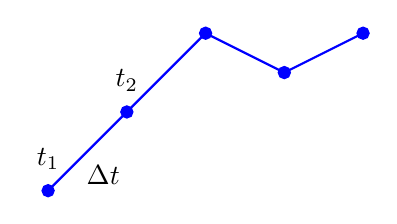
\begin{tikzpicture}
				\draw[thick, color=blue] plot [mark=*,blue, tension=1]
				coordinates{(0, 0) (1, 1) (2, 2) ( 3, 1.5) (4, 2)};
				\node[] at (0, 0.4) {$t_1$};
				\node[] at (0.7, 0.2) {$\Delta t$};
				\node[] at (1, 1.4) {$t_2$};
			\end{tikzpicture}}
			\quad
			\subfigure[Caso continuo: $\Delta t \rightarrow 0$]{
			\begin{tikzpicture}
				\draw[thick, color=blue] plot [smooth, red, tension=1]
				coordinates{(0, 0) (2, 2) ( 3, 1.5) (4, 2)};
			\end{tikzpicture}}
			\caption[Confronto tra caso continuo e discreto]{Traiettoria di una rete di Hopfield nel caso continuo e discreto.}
		\end{figure}
		Per descrivere completamente il comportamento del neurone si deve aggiungere alla \eqref{eq:vi} l'equazione che definisce il valore di attivazione del neurone stesso (vedi Appendice~\ref{cha:sistemi_dinamici}); in questo caso, esso non è più la semplice somma algebrica degli ingressi (caso discreto) ma è una soluzione della seguente equazione differenziale:
		\begin{align*}
			V_i + \tau_i \frac{d V_i}{dt} &= g_\beta \left(\sum_{j} w_{ij} V_j + I_i \right) \\
			\tau_i \frac{d V_i}{dt} &= - V_i + g_\beta(\mu_i) = - V_i + g_\beta \left(\sum_j w_{ji} V_j + I_i \right)
		\end{align*}
		dove $\tau_i$ è una costante ($\tau_i > 0$) e rappresenta la resistenza elettrica. Il sistema raggiunge la stabilità quando il vettore velocità del sistema si azzera $\Delta t = dV_i / dt= 0 \, \forall i$, ovvero quando l'uscita di ogni neurone $V_i$ è uguale a $g_\beta(\mu_i)$:
		\begin{align*}
			V_i = g_\beta(\mu_i)
		\end{align*}
		In maniera del tutto equivalente è possibile esprimere l’equazione di stato non incentrando l’attenzione sulla variazione $V_i$ dello stato nel tempo, quanto sulla variazione $\mu_i$ dell’input netto nel tempo, pervenendo alla seguente equazione:
		\begin{align}
			\mu_i + \tau_i \frac{d\mu_i}{dt} &= \sum_j w_{ij} V_j + I_i = \sum_j w_{ij} g_\beta (\mu_j) + I_i \\
			\tau_i \frac{d\mu_i}{dt} &= -\mu_i + \sum_j w_{ij} g_\beta (\mu_j) + I_i \label{eq:mu}
		\end{align}

		\newpage

		La funzione energia nel modello continuo è simile a quella nel caso discreto ed è così definita:
		\begin{align}
			E = - \frac{1}{2} \sum_i \sum_j w_{ij} V_i V_j + \sum_i \int_0^{V_i} g^{-1}_\beta (V) \, dV - \sum_i I_i V_i
		\end{align}

		Si dimostra ora il teorema di Hopfield nel caso continuo: 
		\begin{thm}[Teorema di Hopfield - Caso Continuo]
			Se $W=W^T$ e $diag(W) = 0$ allora la funzione di energia $E$ è Lyapunoviana per il sistema e quindi $dE / dt \leq 0$, dove l'uguaglianza si ottiene quando il sistema ha raggiunto un punto stazionario.
		\end{thm}

		\begin{proof}[Dimostrazione:]
			È necessario dimostrare che $dE / dt \leq 0$ con uguaglianza quando un punto fisso è stato raggiunto. Si ricorda che solo gli output dei neuroni dipendono dal tempo.\\
	
			Nel calcolo della derivata $dE / dt$, al primo termine è applicata la regola del prodotto mentre per il secondo la regola della catena e il teorema fondamentale del calcolo integrale (vedi Appendice~\ref{cha:matematica}). In questo modo si ottiene:
			\begin{align*}
				\frac{dE}{dt} &= - \frac{1}{2} \sum_i \sum_j w_{ij} \frac{dV_i}{dt} V_j - \frac{1}{2} \sum_i \sum_j w_{ij} V_i \frac{dV_j}{dt} + \sum_i \underbrace{g_\beta^{-1}(V_i)}_\textrm{$= \mu_i$} \frac{dV_i}{dt} - \sum_i I_i \frac{d V_i}{dt} 
			\end{align*}
			Assumendo che $W$ è simmetrica le prime due sommatorie sono uguali e quindi:
			\begin{align*}
				\frac{dE}{dt} &=  - \sum_i \sum_j w_{ij} \frac{dV_i}{dt} V_j + \sum_i \mu_i \frac{dV_i}{dt} - \sum_i I_i \frac{d V_i}{dt} \\
				&= - \sum_i \frac{d V_i}{dt} \underbrace{\left(\sum_j w_{ij} V_j - \mu_i + I_i \right)}_\textrm{$ = \tau_i \frac{d \mu_i}{dt}$} \\
				&= - \sum_i \tau_i \frac{d V_i}{dt} \frac{d \mu_i}{dt}
			\end{align*}
			dove
			\begin{align*}
				\frac{d V_i}{dt} = \frac{d}{dt} \left(g_\beta (\mu_i) \right) = \frac{d \mu_i}{dt} \cdot g'_\beta(\mu_i)
			\end{align*}
			e quindi:
			\begin{align*}
				\frac{dE}{dt} = - \sum_i \tau_i g'_\beta(\mu_i) \left(\frac{d\mu_i}{dt} \right)^2 \leq 0
			\end{align*}
	
			\newpage

			L'ultima disuguaglianza è vera perché $g_\beta$ è monotona crescente quindi la sua derivata $g'_\beta \geq 0$, $\tau_i > 0$ e il quadrato di un numero è sempre positivo. Dunque vale la seguente doppia implicazione:
			\begin{align*}
				\frac{dE}{dt} = 0 \Leftrightarrow \frac{d \mu_i}{dt} = 0
			\end{align*}
			cioè il valore dell'energia nel tempo rimane fisso se e solo se la rete ha raggiunto un punto di equilibrio, ovvero $\mu_i$.
		\end{proof}

		% section modello_di_hopfield_caso_continuo (end)

		\section{Corrispondenza tra i due modelli} % (fold)
		\label{sec:corrispondenza_tra_i_due_modelli}
		Esiste una relazione stretta tra il modello continuo e quello discreto. Si noti che:
		\begin{align*}
			V_i = g_\beta(\mu_i) = g_1(\beta \mu_i) = g(\beta \mu_i)
		\end{align*}
		Da cui si ricava che:
		\begin{align*}
			\mu_i = \frac{1}{\beta} g^{-1} (V_i)
		\end{align*}
		Il secondo termine della funzione energia diventa quindi:
		\begin{align*}
			\sum_i \int_0^{V_i} g^{-1}_\beta (V) \, dV = \frac{1}{\beta} \cdot \sum_i \int_0^{V_i} g^{-1} (V) \, dV 
		\end{align*}
		Ora per $\beta \rightarrow \infty$ il termine diventa trascurabile e la funzione $E$ risulta uguale a quella nel modello discreto.
		\begin{align*}
			E &= - \frac{1}{2} \sum_i \sum_j w_{ij} V_i V_j + \underbrace{\frac{1}{\beta} \cdot \sum_i \int_0^{V_i} g^{-1} (V) \, dV}_\textrm{= 0 per $\beta \rightarrow \infty$}  - \sum_i I_i V_i \\
			&=  - \frac{1}{2} \sum_i \sum_j w_{ij} V_i V_j - \sum_{i=1}^n I_i V_i
		\end{align*}
		Intuitivamente per $\beta \rightarrow \infty$ la funzione diventa sempre più rigida fino a diventare lineare (vedi Figura~\ref{fig:stickiness}). Di conseguenza la funzione energia del caso continuo ora coincide con quella del modello discreto.
		% section corrispondenza_tra_i_due_modelli (end)

		% chapter reti_di_hopfield (end)



